% ----------------------------------------------------
% Literature Review
% ----------------------------------------------------
\documentclass[class=report,11pt,crop=false]{standalone}
% Page geometry
\usepackage[a4paper,margin=20mm,top=25mm,bottom=25mm]{geometry}

% Font choice
\usepackage{lmodern}

% \usepackage{lipsum}

% Use IEEE bibliography style
\bibliographystyle{IEEEtran}

% Line spacing
\usepackage{setspace}
\setstretch{1.20}

% Ensure UTF8 encoding
\usepackage[utf8]{inputenc}

% Language standard (not too important)
\usepackage[english]{babel}

% Skip a line in between paragraphs
\usepackage{parskip}

% For the creation of dummy text
\usepackage{blindtext}

% Math
\usepackage{amsmath}

% Header & Footer stuff
\usepackage{fancyhdr}
\pagestyle{fancy}
\fancyhead{}
\fancyhead[R]{\nouppercase{\rightmark}}
\fancyfoot{}
\fancyfoot[C]{\thepage}
\renewcommand{\headrulewidth}{0.0pt}
\renewcommand{\footrulewidth}{0.0pt}
\setlength{\headheight}{13.6pt}

% Epigraphs
\usepackage{epigraph}
\setlength\epigraphrule{0pt}
\setlength{\epigraphwidth}{0.65\textwidth}

% Colour
\usepackage{color}
\usepackage[usenames,dvipsnames]{xcolor}

% Hyperlinks & References
\usepackage{hyperref}
\definecolor{linkColour}{RGB}{77,71,179}
\hypersetup{
    colorlinks=true,
    linkcolor=linkColour,
    filecolor=linkColour,
    urlcolor=linkColour,
    citecolor=linkColour,
}
\urlstyle{same}

% Automatically correct front-side quotes
\usepackage[autostyle=false, style=ukenglish]{csquotes}
\MakeOuterQuote{"}

% Graphics
\usepackage{graphicx}
\graphicspath{{Images/}{../Images/}}
\usepackage{makecell}
\usepackage{transparent}

% SI units
\usepackage{siunitx}

% Microtype goodness
\usepackage{microtype}

% Listings
\usepackage[T1]{fontenc}
\usepackage{listings}
\usepackage[scaled=0.8]{DejaVuSansMono}

% Custom colours for listings
\definecolor{backgroundColour}{RGB}{250,250,250}
\definecolor{commentColour}{RGB}{73, 175, 102}
\definecolor{identifierColour}{RGB}{196, 19, 66}
\definecolor{stringColour}{RGB}{252, 156, 30}
\definecolor{keywordColour}{RGB}{50, 38, 224}
\definecolor{lineNumbersColour}{RGB}{127,127,127}
\lstset{
  language=Matlab,
  captionpos=b,
  aboveskip=15pt,belowskip=10pt,
  backgroundcolor=\color{backgroundColour},
  basicstyle=\ttfamily,%\footnotesize,        % the size of the fonts that are used for the code
  breakatwhitespace=false,         % sets if automatic breaks should only happen at whitespace
  breaklines=true,                 % sets automatic line breaking
  postbreak=\mbox{\textcolor{red}{$\hookrightarrow$}\space},
  commentstyle=\color{commentColour},    % comment style
  identifierstyle=\color{identifierColour},
  stringstyle=\color{stringColour},
   keywordstyle=\color{keywordColour},       % keyword style
  %escapeinside={\%*}{*)},          % if you want to add LaTeX within your code
  extendedchars=true,              % lets you use non-ASCII characters; for 8-bits encodings only, does not work with UTF-8
  frame=single,	                   % adds a frame around the code
  keepspaces=true,                 % keeps spaces in text, useful for keeping indentation of code (possibly needs columns=flexible)
  morekeywords={*,...},            % if you want to add more keywords to the set
  numbers=left,                    % where to put the line-numbers; possible values are (none, left, right)
  numbersep=5pt,                   % how far the line-numbers are from the code
  numberstyle=\tiny\color{lineNumbersColour}, % the style that is used for the line-numbers
  rulecolor=\color{black},         % if not set, the frame-color may be changed on line-breaks within not-black text (e.g. comments (green here))
  showspaces=false,                % show spaces everywhere adding particular underscores; it overrides 'showstringspaces'
  showstringspaces=false,          % underline spaces within strings only
  showtabs=false,                  % show tabs within strings adding particular underscores
  stepnumber=1,                    % the step between two line-numbers. If it's 1, each line will be numbered
  tabsize=2,	                   % sets default tabsize to 2 spaces
  %title=\lstname                   % show the filename of files included with \lstinputlisting; also try caption instead of title
}

% Caption stuff
\usepackage[hypcap=true, justification=centering]{caption}
\usepackage{subcaption}

% Glossary package
% \usepackage[acronym]{glossaries}
\usepackage{glossaries-extra}
\setabbreviationstyle[acronym]{long-short}

% For Proofs & Theorems
\usepackage{amsthm}

% Maths symbols
\usepackage{amssymb}
\usepackage{mathrsfs}
\usepackage{mathtools}

% For algorithms
\usepackage[]{algorithm2e}

% Spacing stuff
\setlength{\abovecaptionskip}{5pt plus 3pt minus 2pt}
\setlength{\belowcaptionskip}{5pt plus 3pt minus 2pt}
\setlength{\textfloatsep}{10pt plus 3pt minus 2pt}
\setlength{\intextsep}{15pt plus 3pt minus 2pt}

% For aligning footnotes at bottom of page, instead of hugging text
\usepackage[bottom]{footmisc}

% Add LoF, Bib, etc. to ToC
\usepackage[nottoc]{tocbibind}

% SI
\usepackage{siunitx}

% For removing some whitespace in Chapter headings etc
\usepackage{etoolbox}
\makeatletter
\patchcmd{\@makechapterhead}{\vspace*{50\p@}}{\vspace*{-10pt}}{}{}%
\patchcmd{\@makeschapterhead}{\vspace*{50\p@}}{\vspace*{-10pt}}{}{}%
\makeatother

% Tables
\usepackage{multirow}
\usepackage{longtable}
\usepackage{tabularx}
\makenoidxglossaries

\newacronym{radar}{RADAR}{Radio Detection and Ranging}
\begin{document}
\ifstandalone
\tableofcontents
\fi
% ----------------------------------------------------
\chapter{ Power Submodule
(PRMRUV001)\label{ch:power}}
\section{Power Submodule}

In the submodule, it will detail the supply of power to the entire system as a whole. It serves as the heartbeat of the project and is very important. It deals with in a broader scope, the charging and storage of power that can be consumed, as well voltage regulation to a voltage that is suitable for the other submodules that need to draw power.

\section{Requirement Analysis}

In order to design an effective power submodule, analysis of what needs to be achieved in this submodule needs to be carried out extensively. Meeting the user’s requirements are the main objectives. However, in order to meet these requirements well, functional requirements and specifications of the proposed solution needs to be detailed. This can be found below.

\subsection{User Requirements}

These requirements are set out by the client, Sally. In order for the submodule to be a success it would need to meet the requirements. 

\begin{table}
\centering

\begin{tabular}{|>{\raggedright\arraybackslash}p{0.2\linewidth}|>{\raggedright\arraybackslash}p{0.8\linewidth}|}
\hline
\textbf{UR01} & \textbf{Grid Independent} \\
\hline
\textbf{Requirement} & Sally requires the device to charge without the grid mains power supply. \\
\hline
\textbf{Description} & The power system is the heartbeat of the camera trap device, and its awkward placements in nests make it difficult for the device to always be charged using the grid main power supply. Hence, Sally’s requirement for the device to be charged and powered using an alternative power supply method. \\
\hline
\textbf{Refined by} & FR01 \\
\hline

\end{tabular}

\end{table}

 

\begin{table}
\centering

\begin{tabular}{|>{\raggedright\arraybackslash}p{0.2\linewidth}|>{\raggedright\arraybackslash}p{0.8\linewidth}|}
\hline
\textbf{UR02} & \textbf{Reliability} \\
\hline
\textbf{Requirement} & Sally requires a device that has a reliable power supply.  \\
\hline
\textbf{Description} & It was made clear that the monitoring of these birds is very important and so is the data recorded. Hence, it is vitally important that the device continuously has good reliable power supply to operate to avoid data capturing loss. \\
\hline
\textbf{Refined by} & FR02 \\
\hline

\end{tabular}

\end{table}

 

\begin{table}
\centering

\begin{tabular}{|>{\raggedright\arraybackslash}p{0.2\linewidth}|>{\raggedright\arraybackslash}p{0.8\linewidth}|}
\hline
\textbf{UR03} & \textbf{Sizing} \\
\hline
\textbf{Requirement} & Sally requires the device to be light and compact. \\
\hline
\textbf{Description} & The starling birds are very sensitive and particularly do no like foreign objects in their space. Furthermore, the nests that are to be monitored are small and light. Hence, the need for the Power submodule to be as light and compact as possible. \\
\hline
\textbf{Refined by} & FR03 \\
\hline

\end{tabular}

\end{table}

 

\subsection{Functional Requirements}

These requirements are outlined by the designer in order to make the users requirements more detailed. This in turn makes the submodule more coherent and lay out guidelines to follow so that the submodule can be a success.

\begin{table}
\centering

\begin{tabular}{|>{\raggedright\arraybackslash}p{0.2\linewidth}|>{\raggedright\arraybackslash}p{0.8\linewidth}|}
\hline
\textbf{FR01-1} & \textbf{Rechargeable Battery} \\
\hline
\textbf{Requirement} & The system battery needs to be able to support recharging from sources such as solar power. \\
\hline
\textbf{Refines} & UR01 \\
\hline
\textbf{Refined by} & UR01-S01 \\
\hline
\textbf{Verification} & N/A \\
\hline

\end{tabular}

\end{table}

 

\begin{table}
\centering

\begin{tabular}{|>{\raggedright\arraybackslash}p{0.2\linewidth}|>{\raggedright\arraybackslash}p{0.8\linewidth}|}
\hline
\textbf{FR01-2} & \textbf{Solar Panel} \\
\hline
\textbf{Requirement} & The system requires a solar panel as a form of solar power generation to charge the battery. \\
\hline
\textbf{Refines} & UR01 \\
\hline
\textbf{Refined by} & UR01-S02 \\
\hline
\textbf{Verification} & ATP01 \\
\hline

\end{tabular}

\end{table}

 

\begin{table}
\centering

\begin{tabular}{|>{\raggedright\arraybackslash}p{0.2\linewidth}|>{\raggedright\arraybackslash}p{0.8\linewidth}|}
\hline
\textbf{FR02-1} & \textbf{Circuit Protection} \\
\hline
\textbf{Requirement} & The system battery needs to be able to support recharging from sources such as solar power. \\
\hline
\textbf{Refines} & UR01 \\
\hline
\textbf{Refined by} & UR01-S03 \\
\hline
\textbf{Verification} & ATP02, ATP03 \\
\hline

\end{tabular}

\end{table}

 

\begin{table}
\centering

\begin{tabular}{|>{\raggedright\arraybackslash}p{0.2\linewidth}|>{\raggedright\arraybackslash}p{0.8\linewidth}|}
\hline
\textbf{FR02-2} & \textbf{Voltage Conversion} \\
\hline
\textbf{Requirement} & The primary requirement is to provide a steady regulated output voltage of 5V. \\
\hline
\textbf{Refines} & UR02 \\
\hline
\textbf{Refined by} & UR02-S02 \\
\hline
\textbf{Verification} & ATP04 \\
\hline

\end{tabular}

\end{table}

 

\begin{table}
\centering

\begin{tabular}{|>{\raggedright\arraybackslash}p{0.2\linewidth}|>{\raggedright\arraybackslash}p{0.8\linewidth}|}
\hline
\textbf{FR02-4} & \textbf{Voltage ripple} \\
\hline
\textbf{Requirement} & The voltage ripple must be within acceptable limits, ideally as low as 100mV. \\
\hline
\textbf{Refines} & UR02 \\
\hline
\textbf{Refined by} & - \\
\hline
\textbf{Verification} & ATP05 \\
\hline

\end{tabular}

\end{table}

 

\begin{table}
\centering

\begin{tabular}{|>{\raggedright\arraybackslash}p{0.2\linewidth}|>{\raggedright\arraybackslash}p{0.8\linewidth}|}
\hline
\textbf{FR03-1} & \textbf{Size Restriction} \\
\hline
\textbf{Requirement} & The power submodule must fit in the casing dimensions stipulated in the casing submodule. \\
\hline
\textbf{Refines} & UR03 \\
\hline
\textbf{Refined by} & UR03-S01 \\
\hline
\textbf{Verification} & ATP06 \\
\hline

\end{tabular}

\end{table}

 

\section{Design Specifications}

In this chapter, we will specify how the requirements will be met as well as the engineering principles that will be used.

\begin{table}
\centering

\begin{tabular}{|>{\raggedright\arraybackslash}p{0.2\linewidth}|>{\raggedright\arraybackslash}p{0.8\linewidth}|}
\hline
\textbf{UR01-S01} & \textbf{Rechargeable Battery} \\
\hline
\textbf{Detail} & The batteries that will be used will be the 4.2V Lithium ion 18650 8800 mAh battery.  \\
\hline
\textbf{Refines} & FR01-1 \\
\hline
\textbf{Verification} & Battery selection in design choices section. \\
\hline

\end{tabular}

\end{table}

 

\begin{table}
\centering

\begin{tabular}{|>{\raggedright\arraybackslash}p{0.2\linewidth}|>{\raggedright\arraybackslash}p{0.8\linewidth}|}
\hline
\textbf{UR01-S02} & \textbf{Solar Panel} \\
\hline
\textbf{Detail} & The solar panel chosen must be able to provide minimum voltage required to charge the battery.  \\
\hline
\textbf{Refines} & FR01-2 \\
\hline
\textbf{Verification} & N/A \\
\hline

\end{tabular}

\end{table}

 

\begin{table}
\centering

\begin{tabular}{|>{\raggedright\arraybackslash}p{0.2\linewidth}|>{\raggedright\arraybackslash}p{0.8\linewidth}|}
\hline
\textbf{UR02-S01} & \textbf{Circuit Protection} \\
\hline
\textbf{Detail} & The submodule must include an over voltage protection circuit as well as well as a reverse polarity protection circuit in order to protect the components of the submodule.  \\
\hline
\textbf{Refines} & FR02-1 \\
\hline
\textbf{Verification} & ATP02, ATP03 \\
\hline

\end{tabular}

\end{table}

 

\begin{table}
\centering

\begin{tabular}{|>{\raggedright\arraybackslash}p{0.2\linewidth}|>{\raggedright\arraybackslash}p{0.8\linewidth}|}
\hline
\textbf{UR02-S02} & \textbf{Voltage Conversion} \\
\hline
\textbf{Detail} & The submodule will include a buck converter that will regulate the voltage down to a steady 5V.  \\
\hline
\textbf{Refines} & FR02-2 \\
\hline
\textbf{Verification} & ATP7 \\
\hline

\end{tabular}

\end{table}

 

\begin{table}
\centering

\begin{tabular}{|>{\raggedright\arraybackslash}p{0.2\linewidth}|>{\raggedright\arraybackslash}p{0.8\linewidth}|}
\hline
\textbf{UR03-S01} & \textbf{Sizing} \\
\hline
\textbf{Detail} & The submodule must fit in a casing of dimensions 60 x 60 x 80 mm \\
\hline
\textbf{Refines} & FR03-1 \\
\hline

\end{tabular}

\end{table}

\section{Acceptance Test Procedure (ATP’s)}

The acceptance test procedure will ensure that the design meets its intended performance. The procedure involves defining figures of merit, designing experiments to evaluate these metrics, and establishing acceptable performance standards.

\begin{table}
\centering

\begin{tabular}{| l  |l  |>{\raggedright\arraybackslash}p{0.3\linewidth}|>{\raggedright\arraybackslash}p{0.3\linewidth}|}
\hline
\textbf{ATP ID} & \textbf{ATP name} & \textbf{Figures of merit} & \textbf{Test} \\
\hline
\textbf{ATP01} & Solar Panels & Verify that the solar PV panels provide the minimum specified voltage for charging the battery packs.

  & Place Solar under various sun intensities and measure the produced voltages. \\
\hline
\textbf{ATP02} & Over Voltage Protection & Verify that the protection circuits work when they need to. & We can test this by applying a high voltage to the over voltage protection circuit. \\
\hline
\textbf{ATP03} & Reverse Polarity Protection. & Verify that the protection circuits work when they need to. & We can test this by applying a reverse bias current to the reverse polarity circuit. \\
\hline
\textbf{ATP04} & Voltage Regulation & This is about making sure the output voltage stays steady even when things change. We want to know if the converter can keep the voltage where we want it, no matter what's happening. & We'll suddenly change the load to see if the converter can keep the output voltage steady.

We'll watch the output voltage closely and check if it stays within a certain range of the desired voltage. \\
\hline
\textbf{ATP05} & Voltage ripple & We will perform this test to see that the voltage ripple is not exceeding our desired limits. & We can test this by connecting the output of the buck converter to the oscilloscope and using the measure function. \\
\hline
\textbf{ATP06} & Sizing & We will test to see that the power submodule Veroboard can fit in the casing. & We can test this by building our circuits on Veroboard and placing it in the casing. \\
\hline

\end{tabular}

\end{table}

     

\section{Design Choices}

In order to make design choices, we first have to understand how much power is required from the other submodules. This value is no more than 10 W.

\subsection{Battery choice}

There are multiple battery possibilities. However, we need to first calculate the required battery capacity in order to get a good fit. Using the table above we can allocate excess power and work of the required power being 20W. We can also assume we that we want the battery to operate for 12 hours, just enough time for the solar to start again.

We plan on using a five-battery pack rated at 4.2V each. The calculations are as follows:

Since the power required by the system was exaggerated, it is same to say that even with efficiency problems related to a battery, it would still be acceptable.

We can now analyse various batteries at similar rating as seen in the table below:

\begin{table}
\centering

\begin{tabular}{| l | l | l | l |}
\hline
  & \textbf{VRLA AGM Battery} & \textbf{Lead acid battery} & \textbf{Li-ion 18650} \\
\hline
\textbf{Type} & VRLA & LiFePO4  & Lithium ion \\
\hline
\textbf{Rated Voltage (V)} & 12 & 12 & 4.2 \\
\hline
\textbf{Rated Capacity (mAh)} & 7000 & 6000 & 8000 \\
\hline
\textbf{Size (mm)} & 151 x 65 x 95 & 152 x 65 x 97 & 65 x 20 x 20 \\
\hline
\textbf{Cost (R)} & 192 & 499 & 186 (Pack of 5) \\
\hline

\end{tabular}

\end{table}

 From the table above we can conclude our analysis on various types of batteries. With the VRLA AGM Battery, we can see that the rated capacity falls short of the required capacity as well as the rated voltage being too low. The lead acid battery follows the same suit and is very expensive making it a bad match. However, the Li-ion 18650’s seems to be the best match and the battery of choice. It falls withing the required capacity, has a rated voltage of 4.2V which when all are connected in series amount to 21V, and it is relatively affordable.

 

\subsection{Voltage Regulation}

The most crucial part of the power submodule is the voltage regulation. For this specific design, the other submodules only required a regulated voltage of 5V. This means that the voltage from the battery needs to be steeped down to that voltage of 5V. The various ways in which we can achieve that are detailed below:

 

 

\begin{table}
\centering

\begin{tabular}{| l | l | l | l |}
\hline
  & \textbf{L4940V5} & \textbf{CRE1S2405SC} & \textbf{Buck Converter} \\
\hline
\textbf{Input Voltage (V)} & 6.5 – 15 & 24 & 20 \\
\hline
\textbf{Output Voltage (V)} & 5 & 5 & 5 \\
\hline
\textbf{Output Current (A)} & 2.5 & 0.2 & Variable \\
\hline
\textbf{Complexity} & Easy & Easy & Complex \\
\hline
\textbf{Cost} & 28 & 57,07 & 20 \\
\hline

\end{tabular}

\end{table}

 From the table above we can make an inform decision in which methos we are going to use as our step-down regulator. We first analyse the L4940V5 voltage regulator, this does not fit well into the design because it outputs a max current that is high, and the input voltage will require a voltage divider in order for it to meet the specifications stated. The CRE1S2405SC is too expensive to use and also reflects no design thinking behind it. The buck converter using first principles can be tailored to fit any scenario and fits the design of the project best.

Hence, the buck converter using first principles is the best option.

\section{Power Submodule Design}

\subsection{Subsystem Block Diagram}

 \begin{figure}
     \centering
     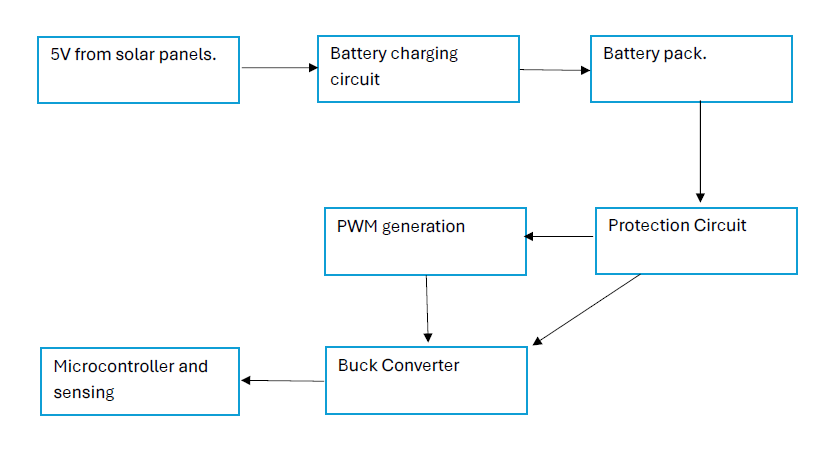
\includegraphics[width=0.5\linewidth]{Power_Flowchart.png}
     \caption{Flowchart of subsystem}
     \label{fig:enter-label1}
 \end{figure}

\subsection{Pulse Width Modulation}

For this part of the submodule a 555 timer will be used to generate a pulse for the switch in the buck converter. The calculations of the parameters are as follows.

The circuit can be found below:
\begin{figure}
    \centering
    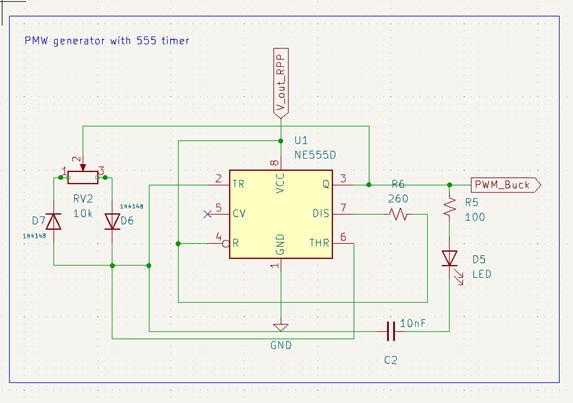
\includegraphics[width=0.5\linewidth]{image.png}
    \caption{PWM generator using a 555 timer.}
    \label{fig:enter-label2}
\end{figure}


\subsection{Buck Converter (Voltage regulation)}

For this project, it is required that the designed system is efficient and can regulate the output voltage to 5V. The circuit parameters can be calculated, as shown below.

To explain how the selection of parameters occurred we will need to have a scenario/problem. 

Let's consider a scenario where we aim to design a DC-DC converter that converts a 20V DC input to a stable 5V DC output. We've chosen a switching frequency of 100 kHz. In addition, we want to maintain a current ripple of 0.5 and a voltage ripple of 10 mV for optimal performance.

 

 

 

 

 

 

 Component selection:

· Inductor value 75 

· Capacitor value 68 

The figure below shows the schematic of the designed circuit:
\begin{figure}
    \centering
    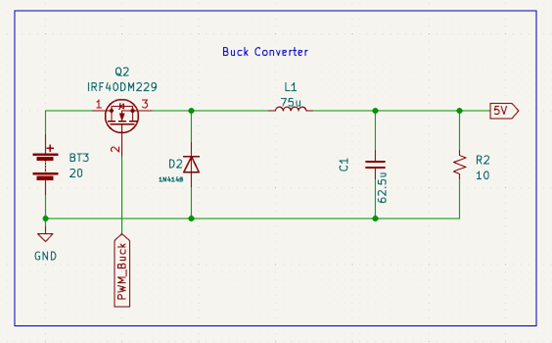
\includegraphics[width=0.5\linewidth]{buck.png}
    \caption{Schematic of buck converter}
\end{figure}

\subsection{Reverse Polarity Protection}

For this design, we simply needed to design a circuit that would provide reverse bias current protection. The simplest way to protect against this happening is to simply use a diode. The circuit can be found below.
\begin{figure}
    \centering
    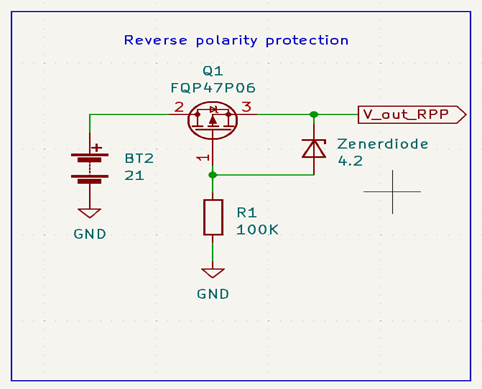
\includegraphics[width=0.5\linewidth]{protection.png}
    \caption{Reverse polarity schematic}
    \label{fig:enter-label3}
\end{figure}

\subsection{Battery Charging Circuit}

For the purpose of the battery charging circuit being able to be charged by solar we took a generic input of Vsupply which is the voltage produced by the solar panels. The schematic of the charging circuit with over voltage protection can be found below.
\begin{figure}
    \centering
    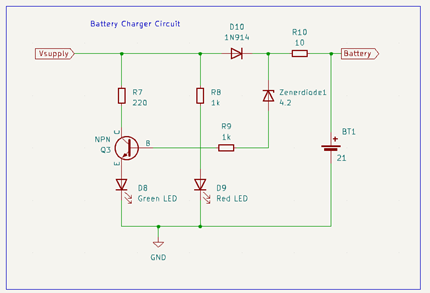
\includegraphics[width=0.5\linewidth]{Battery.png}
    \caption{Battery charging circuit with over voltage protection}
    \label{fig:enter-label4}
\end{figure}

\subsection{Voltage Divider (Receiver)}

For the receiver, there is no need for much protection, just the basics. Hence, it was decided that a voltage regulator with a diode would be perfect for this case. Resistor values were calculated using the voltage divider rule. The schematic of the circuit is below:
\begin{figure}
    \centering
    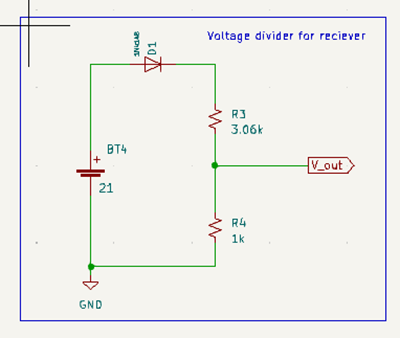
\includegraphics[width=0.5\linewidth]{VoltageDivider.png}
    \caption{Voltage divider for receiver}
    \label{fig:enter-label5}
\end{figure}

\section{Testing and validation}

In this section we will be testing our circuits in order to make sure that they work and perform the way that it is intended to.

\subsection{Pulse width modulation.}

The PWM generator was constructed using the 555 timer and it was then connected to the oscilloscope and the output was captured as seen below.
\begin{figure}
    \centering
    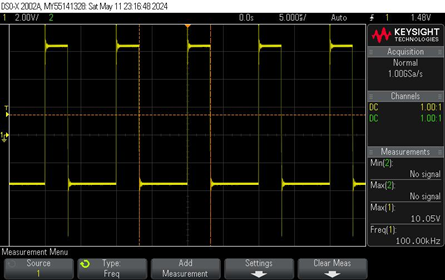
\includegraphics[width=0.5\linewidth]{PWM.png}
    \caption{PWM output}
    \label{fig:enter-label6}
\end{figure}

As seen in the figure, the PWM output works as expected with a duty cycle of 25\%.

\subsection{Protection circuits}

The power protection circuits were then tested. With regards to over voltage protection circuit. We tested this by applying a high voltage to the over voltage protection circuit. The LED switched on to indicate that the voltage was high, and the circuit was then short circuited to ground, cutting of power to the rest of the circuitry.

With regards to the reverse polarity protection circuit. A reverse bias current was applied to the protection circuit. It was observed that the diode was then reverse bias and acted as an open circuit and no current flowed in the circuit. Hence, we can conclude that both protection circuits operated as expected.

\subsection{Voltage divider (Receiver)}

For this circuit, it was fairly simple to test. The voltage regulator was constructed and then tested by measuring the output. The circuit also provided reverse bias protection through the diode. The output was 5V as expected.

\subsection{Buck Converter / Integrated circuits}

To test the buck converter, a 20V supply voltage was applied at the input and the output was then recorded using an oscilloscope. The results were as expected, and the buck converter successfully outputted the desired 5V and shown below.
\begin{figure}
    \centering
    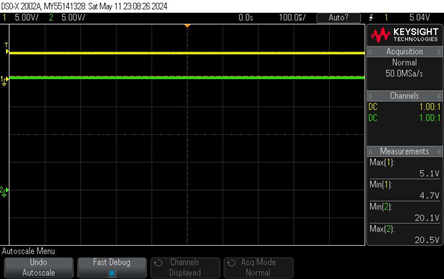
\includegraphics[width=0.5\linewidth]{buckOutput.png}
    \caption{Buck converter output}
    \label{fig:enter-label}7
\end{figure}

\section{ATP Evaluation}

In this section, we revisit the ATP’s and evaluate their extent of success. This evaluation is tabulated below.

\begin{table}
\centering

\begin{tabular}{| l  |l  |l  |>{\raggedright\arraybackslash}p{0.3\linewidth}|}
\hline
\textbf{ATP ID} & \textbf{ATP name} & \textbf{Outcome} & \textbf{Details} \\
\hline
\textbf{ATP01} & Solar Panels & Undecided

  & This ATP test was not completed as a solar panel was not bought due to budget restrictions. \\
\hline
\textbf{ATP02} & Over Voltage Protection & Passed & The over voltage protection circuit worded and opened the circuit when voltage was too high. \\
\hline
\textbf{ATP03} & Reverse Polarity Protection. & Passed & We can test this by applying a reverse bias current to the reverse polarity circuit. \\
\hline
\textbf{ATP04} & Voltage Regulation & Passed  & The buck converter as well as the voltage divider for the receiver outputted 5V and worked as intended. \\
\hline
\textbf{ATP05} & Voltage ripple & Failed & The buck converter had a voltage ripple of 400 mV. \\
\hline
\textbf{ATP06} & Sizing & Failed. & The casing was small and when trying to fit the submodule in, the Veroboard fit but the 5-battery pack did not. \\
\hline

\end{tabular}

\end{table}

 

\section{Conclusion}

In conclusion, the main requirements of the power system submodule have been met and the power submodule was a success. It was a difficult process trying to account for all small details such as voltage ripple being a minimum but in essence the final design worked out well.

% ----------------------------------------------------
\ifstandalone
\bibliography{../Bibliography/References.bib}
\printnoidxglossary[type=\acronymtype,nonumberlist]
\fi
\end{document}
% ----------------------------------------------------